\documentclass{bschlangaul-haupt}
\liLadePakete{formale-sprachen,automaten}
\usepackage{tikz}
\usetikzlibrary{chains,fit,shapes}
\begin{document}

% Info_2021-04-23-2021-04-23_09.35.52 1h50m

%%%%%%%%%%%%%%%%%%%%%%%%%%%%%%%%%%%%%%%%%%%%%%%%%%%%%%%%%%%%%%%%%%%%%%%%
% Theorie-Teil
%%%%%%%%%%%%%%%%%%%%%%%%%%%%%%%%%%%%%%%%%%%%%%%%%%%%%%%%%%%%%%%%%%%%%%%%

\chapter{Linear beschränkte Turingmaschine}

\begin{liQuellen}
\item \cite[Seite 312-317]{hoffmann}
\item \cite{wiki:turingmaschine}
\end{liQuellen}

\section{Simulatoren}

\begin{itemize}
\item \url{https://turingmachinesimulator.com} (online)
\item \url{https://flaci.com/home/} (online)
\item \url{https://www.turing-werkstatt.de/} (Windows)
\end{itemize}

% https://texample.net/tikz/examples/turing-machine-2/
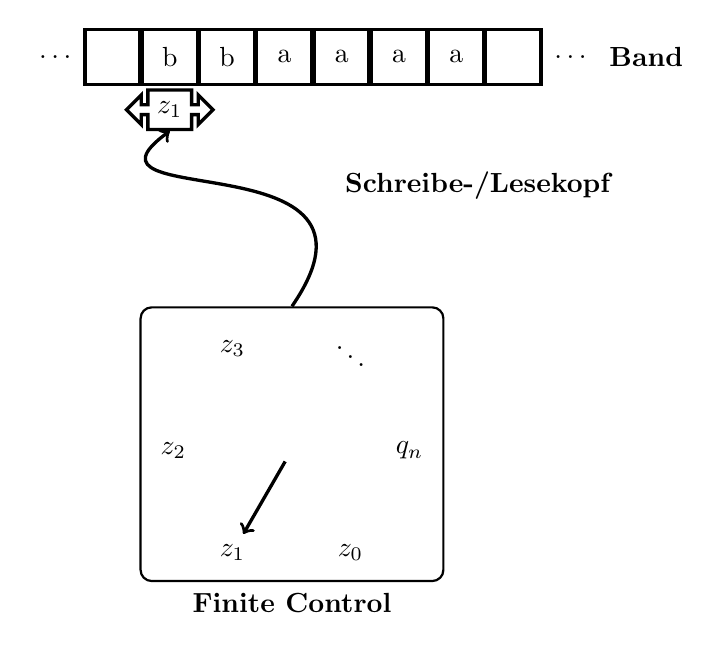
\begin{tikzpicture}
\tikzstyle{every path}=[very thick]

\edef\sizetape{0.7cm}
\tikzstyle{tmtape}=[draw,minimum size=\sizetape]
\tikzstyle{tmhead}=[arrow box,draw,minimum size=.5cm,arrow box
arrows={east:.25cm, west:0.25cm}]

%% Draw TM tape
\begin{scope}[start chain=1 going right,node distance=-0.15mm]
    \node [on chain=1,tmtape,draw=none] {$\ldots$};
    \node [on chain=1,tmtape] {};
    \node [on chain=1,tmtape] (input) {b};
    \node [on chain=1,tmtape] {b};
    \node [on chain=1,tmtape] {a};
    \node [on chain=1,tmtape] {a};
    \node [on chain=1,tmtape] {a};
    \node [on chain=1,tmtape] {a};
    \node [on chain=1,tmtape] {};
    \node [on chain=1,tmtape,draw=none] {$\ldots$};
    \node [on chain=1] {\textbf{Band}};
\end{scope}

%% Draw TM Finite Control
\begin{scope}
[shift={(3cm,-5cm)},start chain=circle placed {at=(-\tikzchaincount*60:1.5)}]
\foreach \i in {z_0,z_1,z_2,z_3,\ddots,q_n}
	\node [on chain] {$\i$};

% Arrow to current state
\node (center) {};
\draw[->] (center) -- (circle-2);

\node[rounded corners,draw=black,thick,fit=(circle-1) (circle-2) (circle-3)
      (circle-4) (circle-5) (circle-6),
			label=below:\textbf{Finite Control}] (fsbox)
		{};
\end{scope}

%% Draw TM head below (input) tape cell
\node [tmhead,yshift=-.3cm] at (input.south) (head) {$z_1$};

%% Link Finite Control with Head
\path[->,draw] (fsbox.north) .. controls (4.5,-1) and (0,-2) .. node[right]
			(headlinetext)
 			{}
			(head.south);
\node[xshift=3cm] at (headlinetext)
			{\textbf{Schreibe-/Lesekopf}};

\end{tikzpicture}

\noindent
Eine deterministische Turingmaschine (TM, DTM) ist ein 7-Tupel
\liTuringMaschine{} ist gegeben durch:

\begin{description}
\item[$Z$]
Eine endliche Menge $Z$ von Zuständen

\item[$\Sigma$]
Ein Eingabealphabet $\Sigma$

\item[$\Gamma$]
Ein Bandalphabet $\Gamma$ mit $\Sigma \subseteq\Gamma$

\item[$\delta$]
Eine partielle Überführungsfunktion
\liTuringUeberfuehrung (L = Links, R = Rechts, N = Neutral)

\item[$z_0$]
Einem Startzustand $z_0 \in Z$

\item[\liTuringLeerzeichen]
Ein Leerzeichen (für das leere Feld) $\liTuringLeerzeichen \in \Gamma \string\ \Sigma$

\item[$E$]
Eine endliche Menge $E \subseteq Z$ von
akzeptierenden Zuständen\footcite[Seite 21]{theo:fs:3}
\end{description}

Die nichtdeterministischen linear beschränkten Turingmaschinen
(LBA = Linear Bounded Automaton) sind Automatenklassen für die
kontextsensitiven Grammatiken/Sprachen.

Ein LBA ist eine Turingmaschine, dessen Band linear beschränkt ist:

\begin{itemize}
\item[Definition 1]

Sie verlässt den Bereich des Bandes auf dem die Eingabe steht nicht.

\item[Definition 2]

Sie kann um einen konstanten Faktor $c$ größeres Band simulieren, sodass
die Turingmaschine höchstens $c \cdot n$ Felder benutzt, wobei $n$ die
Länge des Eingabewortes ist.
\end{itemize}

Eine offene Fragestellung ist, ob jede Sprache, die von einer NLBA
akzeptiert wird, auch durch eine DLBA akzeptiert wird. Sprich:
Akzeptieren DLBA und NLBA die gleiche Sprachklasse
\footcite[Seite 10]{theo:fs:3}

Eine TM terminiert oder hält für ein Wort $w$ genau dann, wenn für
eine gegebene Konfiguration keine Regel definiert ist.

Eine TM akzeptiert ein Wort $w$ genau dann, wenn sie in einem
Endzustand terminiert.

Eine TM mit $k$ Bändern und je einem Schreib-/Lesekopf ist
äquivalent zu einer Einbandturingmaschine. Dabei wird von allen $k$
Bändern zeitgleich je ein Symbol gelesen und jeder der $k$ Köpfe
kann sich unabhängig von den anderen bewegen.
\footcite[Seite 26]{theo:fs:3}

\section{Tabellarische Darstellung der Turingmaschine}

Hierbei sind in der linken Spalte \memph{alle Zustände eingetragen, die
nicht Endzustände sind}, in der obersten Zeile \memph{alle Zeichen des
Bandalphabets}. Die \memph{Tabelleneinträge} selbst geben für den
betreffenden Zustand und das gerade gelesene Bandzeichen als
Arbeitsvorschrift das zu \memph{schreibende Zeichen}, die
\memph{Kopfbewegung} des Lese-/Schreibkopfs und den \memph{Folgezustand}
in Form eines Tripels an.
\liFussnoteUrl{https://info-wsf.de/turingmaschine/}

% Info_2021-04-23-2021-04-23_13.17.40.mp4 3h14min

\section{Mehrbandturingmaschine}

\literatur

\end{document}
